\chapter{Quantum mechanics on a computer}
\begin{itemize}
\item Descriptions of how to perform simulations of atomic systems and Bose–Einstein condensates. Include numerical methods, interaction pictures, Monte–Carlo wavefunction methods and other acquired wisdom that would be relevant to anyone implementing similar simulations.

\item Fourier method: usefulness, use with RK4IP, limitations (i.e. first derivs no good near vortices)


\end{itemize}


    Operators and their matrix representation
    The general case: Need to integrate the equations of motion. What does this mean in a computer? Formal solution of the Schrodinger equation. Is not so formal - can be typed into a programming language thusly: [example code - time ordered product of matrix exponentials].

    Every symbol on the paper has a representation in a computer. State vectors are arrays of complex numbers, operators are matrices - differential operators are no exception. Operators must have a concrete representation, their matrix elements can be computed and then things solved with linear algebra. For discrete degrees of freedom, the matrix representation of the operators may be known, for continuous ones you can find the matrix elements once you define what basis functions you will use [show how]. Or, for the DVR it is a little more subtle (because it's not a basis) but still basically the same process.

\section{The interaction picture}
    \begin{itemize}
        \item Sometimes called a "rotating frame"
        \item Is equivalent to basis change where new basis functions differ by a time-dependent phase factor
        \item Is defined by a time-independent Hamiltonian
        \item This has the effect of moving some time dependence into the operators (demonstrate, by writing some operators with the unitary in front of them. As you can see it is simply a change of basis - but a time-dependent one.)
        \item No need to remain in the same interaction picture - can be redefined arbitrarily often throughout a simulation and state vectors transformed into new basis.
    \end{itemize}

\section{Discrete degrees of freedom}
    \subsection{Unitary integration}
        \subsubsection{Direct exponentiation via diagonalisation of Hamiltonian}
        \begin{itemize}
        \item Unitary - doesn't mean it's accurate but means it won't explode. Great for the bits of your simulation that are explosion-prone but don't matter (like regions of space where the wavefunction is near zero but the potential is large or steep)
        \item error is order [whatever it is] per timestep, not great compared to RK4
        \item can be combined with RK4 to improve accuracy (see later subsection)
        \end{itemize}
        \subsubsection{Approximate exponentiation by operator product}

        [Comment in this section how the approximate total unitary can be used at each timestep to define an interaction picture, and the remaining dynamics simulated with RK4 like RKILIP does in the spatial basis. Interaction pictures are really useful!]
\section{Continuous degrees of freedom}
    \begin{itemize}
        \item Have to be discretised in some way to simulate on a computer - need basis functions. Often a spatial basis is used. Any spatial basis must be combined with assumptions about what the wavefunction is doing at points in between the basis points, in order to define differential operators. Finite differences approximates wavefunction as low-order polynomial in between points (is this equivalent to a polynomial \emph{basis}? Probably not.). Fourier method assume the Fourier series of the wavefunction at the given points can be used to interpolate between points (or the wavefuntion can be Fourier transformed and calculations can be done directly in the Fourier basis). DVR is not actually a spatial basis despite appearances. It assumes the wavefunction is a sum of polynomial 'shape functions', but these shape functions are not basis functions as they are not orthonormal. This is why it is called a representation rather than a basis. Regardless, the shape functions can be used to define an interpolation of the wavefunction between points and thus define differential operators.

    \end{itemize}
    \subsection{Finite differences}
        Show a matrix representation of a few different finite differences, to show that differential operators really are just matrices. They approximate the function as low-order polynomials about each point. You can take them to arbitrarily high order.
    \subsection{The Fourier basis}
        Because of properties of Fourier transforms, derivitives can be taken in Fourier space as simple multiplication. This is essentially because differential operators are diagonal in the Fourier basis. So you can use this fact to define a differential operator in the spatial basis [show matrix] ...or, you could just implement it with Fourier transforms, since FFTs are faster than matrix-vector multiplication ($O(n \log (n)$) rather than $O(n^2)$)
        \subsubsection{Split operator method}
            \begin{itemize}
            \item Equivalent to approximate exponentiation via operator product with the discrete case
            \end{itemize}
    \subsection{Harmonic oscillator basis functions}

\section{Finding groundstates}
\subsection{Imaginary time evolution}
\subsection{Successive over-relaxation}
\subsection{Generalisation to excited states via Gram–Schmidt orthonormalisation}
Directly diagonalising a Hamiltonian can be costly in a spatial basis. Another approach is to find the groundstate using one of the above techniques, and then repeat the process, subtracting off the wavefunction's projection onto the already found groundstate at every step. This yields the lowest energy state that is orthogonal to the first - i.e the first excited state. Repeating the process, but subtracting off \emph{both} eigenstates found so far, then yields the second excited state and so forth. This is simply the Gram-Schmidt process for finding orthonormal vectors, with the additional step of relaxing each vector to the lowest possible energy for each one - this ensures the eigenstates of the Hamiltonian are produced, rather than a different orthogonal basis. Extra conditions can be imposed on the wavefunction at each relaxation step in order to obtain particular solutions in the case of degenerate eigenstates. For example, a phase winding can be imposed in order to obtain a particular harmonic oscillator state - otherwise this process produces an arbitrary superposition of basis states that have equal energy.

\section{The finite-element discrete variable representation}

[explanation of how it works, comparison of implementation with RSP4 vs something like RK4. RK4 is more general purpose, method does not need to be modified for different Hamiltonians. Main limitation is inability to factor out fast dynamical phases, see RK4ILIP for solution to this. MPI implementation and scaling properties with increasing cores. Superscaling at low number of cores. Mention how my implementation can tolerate high network latency due to early sending od data before all local computations are complete. Mention that it is ripe for GPU processing. Limitations: vulnerable to Runge's phenomenon for sharp potentials. Can't increase the order of the polynomials much because small spacing at the edges requires tiny timesteps. Possible solution: pre-conditioning the potential to be an approximation better representable in the DVR basis.]


\section{Fourth order Runge-Kutta in an instantaneous local interaction picture}
\sectionmark{RK4 in an instantaneous local interaction picture}

TODO:
\begin{itemize}
\item Cite RSP stuff, talk about how this is ideal for FEDVR
\item talk about how this solves the last remaining reason why RK4 can't reliably be used over those difficult to implement unitary methods (well, they're difficult when the Hamiltonian isn't super simple)
\item spruik benefits of RK4 ``workhorse" etc, no special transformations of DE required, good accuracy per step etc.
\end{itemize}

Consider the differential equation for the components of a state vector $\ket{\psi(t)}$ in a particular basis with basis vectors $\ket{n}$. This might simply be the Schrödinger equation, or perhaps some sort of nonlinear or other approximate, effective or phenomenological equation not corresponding to pure Hamiltonian evolution. Though they may have additional terms, such equations are generally of the form:
\begin{align}\label{eq:real_imag}
\dv t \braket{n}{\psi(t)} = -\frac i \hbar \sum_m \matrixel{n}{\hat H(t)}{m} \braket{m}{\psi(t)},
\end{align}
where $\matrixel{n}{\hat H(t)}{m}$ are the matrix elements in that basis of the Hamiltonian $\hat H(t)$, which in general can be time dependent, or even a function of $\ket{\psi(t)}$, depending on the exact type of equation in use. Often, and if the basis is chosen well, this type of evolution is dominated by simple dynamical phase evolution, that is, $\hat H(t)$ is almost diagonal in the $\ket{n}$ basis. A transformation into an \emph{interaction picture} (IP) is commonly used to treat this part of the evolution analytically, before solving the remaining dynamics with further analytics or numerics. For numerical methods, integration in the interaction picture allows one to take larger integration timesteps, as one does not need to resolve the fast oscillations around the complex plane due to this dynamical phase.

Choosing an interaction picture typically involves diagonalising the time independent part of a Hamiltonian, and then proceeding in the basis in which that time-independent part is diagonal. However, often one has a good reason to perform computations in a different basis\footnote{such as a spatial basis which allows for partitioning the integration region over multiple nodes on a cluster or cores on a GPU}, and transforming between bases may be computationally expensive (involving large matrix-vector multiplications). Furthermore, the Hamiltonian may change sufficiently from one part of the computation to another that the original time-independent Hamiltonian to no longer dominates the dynamics at later times. In both these cases it would still be useful to factor out the time-local oscillatory dynamics in whichever basis is being used, in order to not have to take unreasonably small timesteps.

To that end, we decompose $H(t)$ into diagonal and non-diagonal (in the $\ket{n}$ basis) parts at each moment in time:
\begin{align}
\hat H(t) = \hat H_{\mathrm{diag}}(t) + \hat H_{\mathrm{nondiag}}(t)
\end{align}
and we use the diagonal part at a specific time $t=t^\prime$ to define a time-independent Hamiltonian:
\begin{align}\label{eq:H0def}
 \hat H_0^{t^\prime} = \hat H_{\mathrm{diag}}(t^\prime),
\end{align}
which is diagonal in the $\ket{n}$ basis. We then use then use $\hat H_0^{t^\prime}$ to define an interaction picture state vector $\ket{\psi_I^{t^\prime}(t)}$:
\begin{align}\label{eq:IP_definition}
\ket{\psi_I^{t^\prime}(t)} = \e^{\frac i \hbar \hat H_0^{t^\prime}(t - t^\prime)}\ket{\psi(t)},
\end{align}
which obeys the differential equation:
\begin{align}\label{eq:IPDE}
\dv t \ket{\psi_I^{t^\prime}(t)}
    = \e^{\frac i \hbar \hat H_0^{t^\prime}(t - t^\prime)}\dv t \ket{\psi(t)}
      + \frac i\hbar \hat H_0^{t^\prime}\ket{\psi_I^{t^\prime}(t)},
\end{align}
where:
\begin{align}\label{eq:backtransform}
\ket{\psi(t)} = \e^{-\frac i \hbar \hat H_0^{t^\prime}(t - t^\prime)}\ket{\psi_I^{t^\prime}(t)}
\end{align}
is the original Schrödinger picture (SP) state vector.

This transformation is exact, no approximations or assumptions have been made. If indeed the dynamics of $\ket{\psi(t)}$ in the given basis are dominated by fast oscillating dynamical phases, then solving the differential equation for $\ket{\psi_I^{t^\prime}(t)}$ should allow one to take larger integration timesteps than solving (\ref{eq:real_imag}) directly. And if not, then it should do no harm other than the (small) computational costs of computing some extra exponentials.

Equation (\ref{eq:IP_definition}) defines an \emph{instantaneous} interaction picture, in that it depends on the dynamics at a specific time $t=t^\prime$, and can be recomputed repeatedly throughout a computation in order to factor out the fast dynamical phase evolution even as the oscillation rates change over time. It is \emph{local} in that $H_0^{t^\prime}$ is diagonal in the $\ket{n}$ basis, which means that transformations between Schrödinger picture and interaction picture state vectors involves ordinary elementwise exponentiation of vectors, rather than matrix products. Thus (\ref{eq:IP_definition}), (\ref{eq:IPDE}) and (\ref{eq:backtransform}) become:

\begin{align}\label{eq:IP_definition_components}
\braket{n}{\psi_I^{t^\prime}(t)} = \e^{ i \omega_n^{t^\prime}(t - t^\prime)}\braket{n}{\psi(t)},
\end{align}
\begin{align}\label{eq:IPDE_components}
\dv t \braket{n}{\psi_I^{t^\prime}(t)}
    = \e^{i \omega_n^{t^\prime}(t - t^\prime)}\dv t \braket{n}{\psi(t)}
      + i\omega_n^{t^\prime}\braket{n}{\psi_I^{t^\prime}(t)},
\end{align}
and:
\begin{align}\label{eq:backtransform_components}
\braket{n}{\psi(t)} = \e^{-\omega_n^{t^\prime}(t - t^\prime)}\braket{n}{\psi_I^{t^\prime}(t)},
\end{align}
where we have defined:
\begin{align}\label{eq:omega}
\omega_n^{t^\prime} = \frac 1\hbar \hat H_0^{t^\prime}
\end{align}
This is in contrast to RK4IP [cite], in which the interaction picture uses the Fourier basis and transforming to and from it involves fast Fourier transforms. RK4IP was developed to augment computations in which FFTs were already in use for evaluating spatial derivatives, and so its use of FFTs imposed no additional cost. Even if one is using FFTs already, our method is still useful for avoiding fast oscillating dynamical phases that are not due to the kinetic term (which is the term of the Hamiltonian that RK4IP takes as its $H_0$). We compare results of the two methods below [TODO].

\subsection{Algorithm}
Our idea is to use (\ref{eq:IP_definition}) to define a new interaction picture at the beginning of each fourth-order Runge–Kutta (RK4) integration timestep. The differential equation and initial conditions supplied to the algorithm are in the ordinary Schrödinger picture, and the interaction picture is used only within a timestep, with the Schrödinger picture state vector returned at the end of each timestep. Thus differential equations need not be modified in any way compared to if ordinary RK4 were being used, and the only modification to calling code required is for a function to compute and return $\omega_n^{t^\prime}$ be provided.

Below is the resulting algorithm for performing one integration timestep. It takes as input the time $t_0$ at the start of the timestep, the timestep size $\upDelta t$, the components $\psi_0^{(n)}$ of the state vector at the start of the timestep, a function $F(t, \psi^{(n)})$ which takes a time and (the components of) a state vector and returns the time derivative for each component, and a function $G(t, \psi^{(n)})$ which takes the same inputs and returns the interaction picture oscillation frequency $\omega_{t}$ for each component at a particular time.

For example, for the case of the Gross-Pitaevskii equation in the spatial basis $\psi(\vec r, t) = \braket{\vec r}{\psi(t)}$, these would be:
\begin{align}\label{eq:GPE}
F(t, \psi(\vec r, t)) = -\frac i \hbar\left[-\frac{\hbar^2}{2m}\nabla^2 + V(\vec r, t) + |\psi(\vec r, t)|^2\right]\psi(\vec r, t),
\end{align}
and
\begin{align}
G(t, \psi(\vec r, t)) = V(\vec r, t) + |\psi(\vec r, t)|^2.
\end{align}

Note that each symbol with a superscript $^{(n)}$ denotes the entire set over all $n$, subscripts denote the different stages of RK4, and all operations are elementwise,. The only opportunity for non-elementwise operations may occur within $F$, which contains the details of any couplings between basis states for whatever system of equations is being solved, for example, using Fast Fourier transforms or finite differences to evaluate the Laplacian in (\ref{eq:GPE}).


\begin{algorithmic}[1]
\linespread{1.5}
\footnotesize
\Function{$\mathrm{RK4ILIP}$}{$t_0$, $\upDelta t$, $\psi_0^{(n)}$, $F$}
    \State $f_1^{(n)} \gets F(t_0, \psi_0^{(n)})$
    \Comment{First evaluation of Schrödinger picture DE}
    \State $\omega^{(n)} \gets G(t_0, \psi_0^{(n)})$
    \Comment{Oscillation frequencies: $\hbar\omega^{(n)} = \matrixel{n}{\hat H_{\mathrm{diag}}(t_0)}{n}$}
    \State $k_1^{(n)} \gets f_1^{(n)} + i\omega^{(n)}\psi_0^{(n)}$
    \Comment{Evaluate (\ref{eq:IPDE_components}) with $t-t^\prime=0$}
    \State $\phi_1^{(n)} \gets \psi_0^{(n)} + k_1^{(n)} \frac{\upDelta t}{2}$
    \Comment{First RK4 estimate of IP state vector, at $t=t_0 + \frac{\upDelta t}{2}$}
    \State $\psi_1^{(n)} \gets \e^{-i\omega^{(n)}\frac{\upDelta t}{2}}\phi_1^{(n)}$
    \Comment{Convert first estimate back to SP}
    \State $f_2^{(n)} \gets F(t_0 + \frac{\upDelta t}{2}, \psi_1^{(n)})$
    \Comment{Second evaluation of Schrödinger picture DE}
    \State $k_2^{(n)} \gets \e^{i\omega^{(n)}\frac{\upDelta t}{2}}f_2^{(n)} + i\omega^{(n)}\phi_1^{(n)}$
    \Comment{Evaluate (\ref{eq:IPDE_components}) with $t-t^\prime=\frac{\upDelta t}{2}$}
    \State $\phi_2^{(n)} \gets \psi_0^{(n)} + k_2^{(n)} \frac{\upDelta t}{2}$
    \Comment{Second RK4 estimate of IP state vector, at $t=t_0 + \frac{\upDelta t}{2}$}
    \State $\psi_2^{(n)} \gets \e^{-i\omega^{(n)}\frac{\upDelta t}{2}}\phi_2^{(n)}$
    \Comment{Convert second estimate back to SP}
    \State $f_3^{(n)} \gets F(t_0 + \frac{\upDelta t}{2}, \psi_2^{(n)})$
    \Comment{Third evaluation of Schrödinger picture DE}
    \State $k_3^{(n)} \gets \e^{i\omega^{(n)}\frac{\upDelta t}{2}}f_3^{(n)} + i\omega^{(n)}\phi_2^{(n)}$
    \Comment{Evaluate (\ref{eq:IPDE_components}) with $t-t^\prime=\frac{\upDelta t}{2}$}
    \State $\phi_3^{(n)} \gets \psi_0^{(n)} + k_3^{(n)} \upDelta t$
    \Comment{Third RK4 estimate of IP state vector, at $t=t_0 + \upDelta t$}
    \State $\psi_3^{(n)} \gets \e^{-i\omega^{(n)}\upDelta t}\phi_3^{(n)}$
    \Comment{Convert third estimate back to SP}
    \State $f_4^{(n)} \gets F(t_0 + \upDelta t, \psi_3^{(n)})$
    \Comment{Fourth evaluation of Schrödinger picture DE}
    \State $k_4^{(n)} \gets \e^{i\omega^{(n)}\upDelta t}f_4^{(n)} + i\omega^{(n)}\phi_3^{(n)}$
    \Comment{Evaluate (\ref{eq:IPDE_components}) with $t-t^\prime=\upDelta t$}
    \State $\phi_4 \gets
            \psi_0 + \frac{\upDelta t}{6}\left(k_1^{(n)} + 2k_2^{(n)} + 2k_3^{(n)} + k_4^{(n)}\right)$
    \Comment{Fourth RK4 estimate, at $t=t_0 + \upDelta t$}
    \State $\psi_4^{(n)} \gets \e^{-i\omega^{(n)}\upDelta t}\phi_4^{(n)}$
    \Comment{Convert fourth estimate back to SP}
    \State \Return $\psi_4^{(n)}$
    \Comment{Return the computed SP state vector at $t=t_0 + \upDelta t$}
\EndFunction
\end{algorithmic}


\subsection{Results}

\begin{itemize}
\item compare with ordinary RK4, RK4IP and split-step for the 2D harmonically trapped turbulent BEC example. Increase timestep until they all break and make a plot of energy error over the 100ms simulation as a function of timestep. Expect all methods to be about the same, with RK4IP being slightly lower error but not much. RK4IP will not blow up at large timesteps, but that doesn't mean it's accurate. Comment on the fact that larger timesteps with RK4IP or split step might be stable in that they don't cause the simulation to blow up, but that timesteps larger than that dictated by the dispersion relation necessarily miss some of the nonlinear dynamics, leading to that inaccuracy. This is ok if you are close to a groundstate such that the dynamics are all pretty linear, but it's not OK for vortices and the like. To demonstrate this, perhaps repeat the comparison with a BEC full of sound waves but no vortices.

\item compare the three methods for the case of an anharmonic trap, increasing the degree of the polynomial $V = r^\alpha$. Show that as soon as a potential higher than a few times the chemical potential exists anywhere in the simulation region, ordinary RK4 requires much smaller timesteps (than that give by the dispersion relation) to not blow up. Split step would probably still do fine.

\item but what about when the equation is more complicated? There is no split step method that can do a rotating frame without colossal matrix-vector products, since the rotation terms are not diagonal in either the spatial or the Fourier basis. This is where RK4ILIP should shine, because it doesn't care how complicated your Hamiltonian is. So compare the RK4 methods for the case of an  anharmonic trap in a rotating frame. (include a harmonic trap that exactly cancels the centrifugal potential, in addition to the anharmonic trap, as per Tapio's suggestion).
\end{itemize}

\begin{align}
\ \mathbfit{\theta} a \theta \\
i\hbar\pdv t \Psi(\vec r, t) = \left[-\frac{\hbar^2}{2m}\nabla^2 + V_{\mathrm{eff}}\right]\psi(\vec r, t)
\end{align}
extaminable
The\ quick\ brown\ fox\ jumped\ over\ the\ lazy\ dog
\emph{The\ quick\ brown\ fox\ jumped\ over\ the\ lazy\ dog}
\begin{align}
\mathrm{The\ quick\ brown\ fox\ jumped\ over\ the\ lazy\ dog}\\
The\ quick\ brown\ fox\ jumped\ over\ the\ lazy\ dog\\
V = \frac43\pi r^3\\
V = \frac43\uppi r^3\\
V = \frac43\itpi r^3\\
\e^{x^2/{2\sigma^2}}\\
\e^{ i x^2/{2\sigma^2}}\\
\pdv{f}{x} = \frac{\partial f}{\partial x}
\end{align}


\afterpage{
    \newgeometry{left=2.54cm,bottom=1.5in,right=2.54cm,top=1.5in}
    \begin{figure}[t]
        \centerfloat
        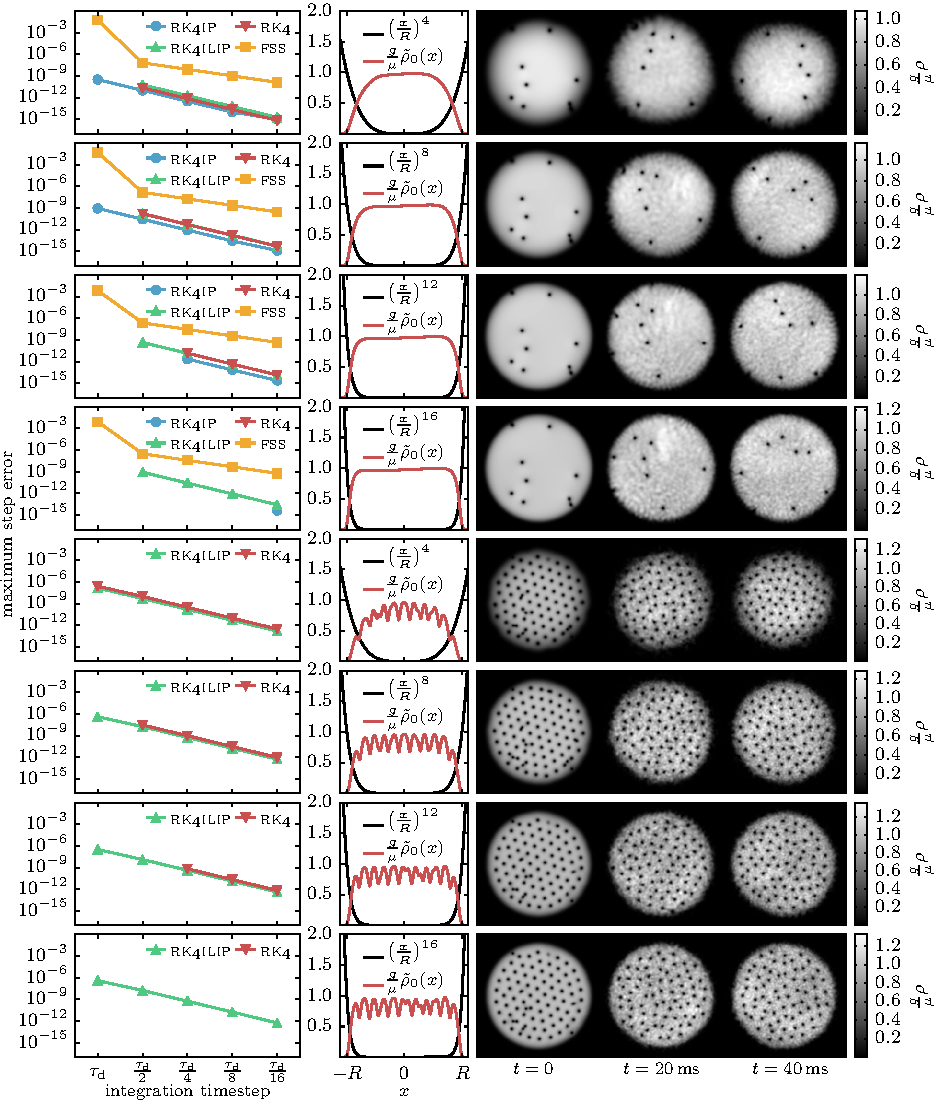
\includegraphics{figures/numerics/rk4ilip_results.pdf}
        \caption{
            Lorem ipsum dolor sit amet, consectetur adipiscing elit. Cras consequat convallis lobortis. Fusce posuere, nibh non sodales dignissim, neque mauris eleifend augue, et gravida nunc magna quis mi. Phasellus cursus finibus convallis. In tempor purus quis urna posuere efficitur. Aenean posuere aliquet ligula at ultrices. Praesent feugiat lacinia enim, in aliquam turpis vestibulum non. Quisque diam lectus, malesuada vel imperdiet sit amet, posuere pretium ante. Aliquam vestibulum nisi in ipsum posuere pellentesque. Lorem ipsum dolor sit amet, consectetur adipiscing elit.}
        \label{fig:rk4ilip_results}
    \end{figure}
    \restoregeometry
}

\lipsum\footnote{ Lorem ipsum dolor sit amet, consectetur adipiscing elit. Cras consequat convallis lobortis. Fusce posuere, nibh non sodales dignissim, neque mauris eleifend augue, et gravida nunc magna quis mi. Phasellus cursus finibus convallis. In tempor purus quis urna posuere efficitur. Aenean posuere aliquet ligula at ultrices. Praesent feugiat lacinia enim, in aliquam turpis vestibulum non. Quisque diam lectus, malesuada vel imperdiet sit amet, posuere pretium ante. Aliquam vestibulum nisi in ipsum posuere pellentesque. Lorem ipsum dolor sit amet, consectetur adipiscing elit. Cras consequat convallis lobortis. Fusce posuere, nibh non sodales dignissim, neque mauris eleifend augue, et gravida nunc magna quis mi. Phasellus cursus finibus convallis. In tempor purus quis urna posuere efficitur. Aenean posuere aliquet ligula at ultrices.}\lipsum\lipsum\footnote{ Lorem ipsum dolor sit amet, consectetur adipiscing elit. Cras consequat convallis lobortis. Fusce posuere, nibh non sodales dignissim, neque mauris eleifend augue, et gravida nunc magna quis mi. Phasellus cursus finibus convallis. In tempor purus quis urna posuere efficitur. Aenean posuere aliquet ligula at ultrices. Praesent feugiat lacinia enim, in aliquam turpis vestibulum non. Quisque diam lectus, malesuada vel imperdiet sit amet, posuere pretium ante. Aliquam vestibulum nisi in ipsum posuere pellentesque. Lorem ipsum dolor sit amet, consectetur adipiscing elit. Cras consequat convallis lobortis. Fusce posuere, nibh non sodales dignissim, neque mauris eleifend augue, et gravida nunc magna quis mi. Phasellus cursus finibus convallis. In tempor purus quis urna posuere efficitur. Aenean posuere aliquet ligula at ultrices.}\lipsum\lipsum\footnote{ Lorem ipsum dolor sit amet, consectetur adipiscing elit. Cras consequat convallis lobortis. Fusce posuere, nibh non sodales dignissim, neque mauris eleifend augue, et gravida nunc magna quis mi. Phasellus cursus finibus convallis. In tempor purus quis urna posuere efficitur. Aenean posuere aliquet ligula at ultrices. Praesent feugiat lacinia enim, in aliquam turpis vestibulum non. Quisque diam lectus, malesuada vel imperdiet sit amet, posuere pretium ante. Aliquam vestibulum nisi in ipsum posuere pellentesque. Lorem ipsum dolor sit amet, consectetur adipiscing elit. Cras consequat convallis lobortis. Fusce posuere, nibh non sodales dignissim, neque mauris eleifend augue, et gravida nunc magna quis mi. Phasellus cursus finibus convallis. In tempor purus quis urna posuere efficitur. Aenean posuere aliquet ligula at ultrices.}\lipsum



